\chapter{The Framework}

\section{From Requirements to Monitors}

The components structure of the developed framework is shown in Fig. \ref{fig:tool}.
\begin{figure}[!h]
	\centering 
     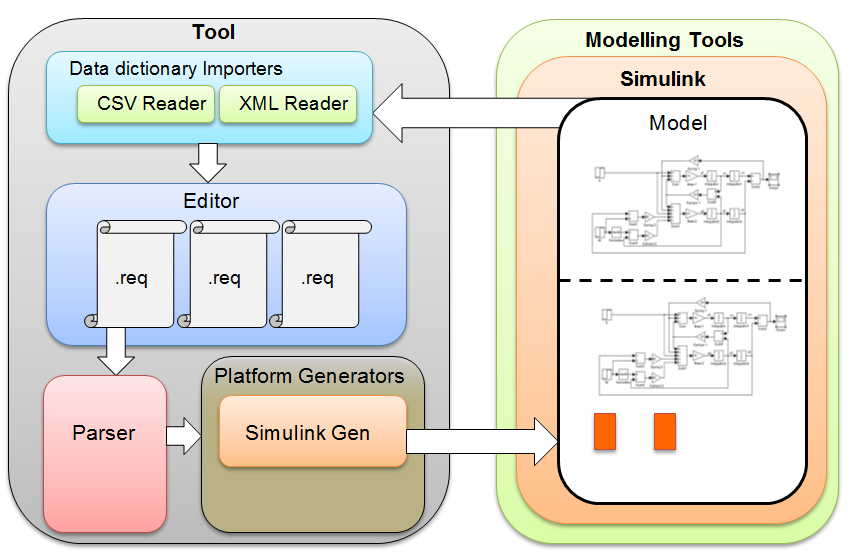
\includegraphics[width=.9\textwidth]{Figs/tool.PNG} 
     \caption{Requirement Framework} 
     \label{fig:tool} 
\end{figure}
\paragraph{Model to Tool} The tool cooperates with a modeling environment through two actions. The first consists of using a model reader to import the list of all model's signals and parameters into a data dictionary. This allows to write requirement referring entities directly with the same names as they are specified in the model. In addition to names, the import phase concur to gather information about data types, boundary values and measuring units.
\paragraph{Tool to Model} The second actions consists of populating the model with monitors generated out of the requirements. Such action is strictly dependent on the platform on which the model is defined. For this reason the tool has been designed to be as flexible as possible, by providing a set of \textit{{Platform Generators}} modules, each one for a specific target platform. In general, in order to ease its task, a platform generator could be supported with some platform libraries enclosing either operators or atomic instructions. In the case of Simulink the produced result is a script which, once executed, adds new requirements blocks to the provided model.
\paragraph{The Editor} In order to write requirements the tool offers a smart editor. It provides the most common user relieving features, such as the context-aware syntax completion ad coloring. Requirements are written according to a specific loose syntax, which is basically equivalent to an ordered sequences of natural language keywords. Even in this case, due to the large variability of possible syntaxes, the tool shows flexibility and provide support for syntax updates with very low effort.
\paragraph{The Parser} The syntax accepted by the editor is not as formal as a the one of a programming language, this complicates not a little the translation of a requirement as it is written. Therefore, before being delivered to a platform generator, the content of a requirement document is transformed into a syntax tree by means of a \textit{Mid Level Parser}. This action, although adds a further step to the synthesis process, ease the task of the platform generator since restructures its input in order to be programmatically analyzable.
\paragraph{} Following sections describe in depth all the components. As first version the tool support interactions only with Simulink, which is one of the most used modeling tools. However, for the sake of completeness, during explanation particular attention will be pose to emphasize all techniques adopted, during the development, to enforce extensibility of the tool. For this reason, also a brief survey of common Design Patterns will be conduced in \ref{sec:designpattern}.

\subsection{Syntax Definition}
\label{ssec:editorsyn}

The syntax of a requirement document has been developed in order to define requirements as contracts, the guarantee will be referred as an assertion, while the concept of precondition has not been explicitly used.
\par The grammar of the syntax is proposed as a list of recursive rules, each mandatory rule is enclosed within angular parentheses, while an optional one is enclosed within square parentheses. At the end of the recursion, rules are primitive, in the sense that they could be expressed through primitive data types (String, Integer, \dots). 
\noindent
\\
The entire syntax is defined as follow
\begin{lstlisting}[language=C]
Requirement Document = <Requirement List>
Requirement List = <Requirement>[Requirement List]
Requirement = <Header><Assumptions Section><Assertions Section>
Header = <ID><Title>
ID = 'R'<Requirement Number>
Requirement Number = <unsigned int>['.'Requirement Number]
Title = <string>
Assumption Section = <"ASSUMPTION"><Assumption List>
Assumption List = <Assumption>["AND" Assumption List]
Assumption = <Comparison statement> | <Signal Generator> | <Reference>
Comparison Statement = <Signal ID><Intermission><Comparison-op><SPV>
SPV = <Signal ID> | <Parameter ID> | <Value>
PV = <Parameter ID> | <Value>
Signal ID = FROM_DATA_DICT
Parameter ID = FROM_DATA_DICT
Value = <double>
Intermission = [Free-text]<"is" | "not">[Free-text]
Free-text = <string>
Comparison-op = <L_EQ> | <G_EQ> | <EQ>
L_EQ = <"less than">["or" EQ]
G_EQ = <"greater than">["or" EQ]
EQ = <"equal to">
Signal Generator = <Signal ID><"is"><Generator Type>
Generator Type = <Step> | <Ramp>
Step = <Step Type><"with amplitude"><PV><"beginning in"><PV>
Step Type = <"step"> | <"downstep">
Ramp = <"ramp with amplitude"><PV><",duration"><PV><"beginning in"><PV>
Reference = <Signal ID><"is reference">
Assertion Section = "ASSERTION"<Assertion List>
Assertion List = <Assertion>["AND" Assertion List]
Assertion = <Control Assertion>
Control Assertion = <Overshoot> | <Undershoot> | <Rise_Fall Time> |       <Settling Time>
Overshoot = <Signal ID><"overshoot shall be less than"><PV>
Undershoot = <Signal ID><"undershoot shall be greater than"><PV>
Rise_Fall Time = <Signal ID><"shall"><Rise_Fall><"from"><PV><"in less than"><PV>
Rise_Fall = <"rise"> | <"fall">
Settling Time = <Signal ID><"time to settle to"><PV><"shall be less        than"><PV>
\end{lstlisting}

\section{Support from Modeling Environment}

The cooperation of the requirements tool with a modeling environment could be easier if from the latter's side are provided some utilities. A good practice when writing requirements is to fill a data dictionary with system's components names and always refer them with that. To enforce the use of a data dictionary a modeling environment may offer the capability to partially generate it by exporting all entities in the model. From the other side, the process of auto-generate monitors for a targeted modeling environment can be lightened if the requirement tool could make use of built-in libraries. The libraries used to provide support for monitors generation have been already described in \citep{bals2017}. Since this thesis is meant as continuation of that work such libraries are reanalyzed, possibly providing further details, also in this context. Next sections explore in a more detailed way these utilities, providing also examples in the case of Simulink.

\subsection{Signal Exporter}

A Simulink model can be view as a collection of connected blocks, where each connecting line represents a signal. In complex models the number of signals is in the order of thousands. The environment allow to name every signal but, for the sake of practicality, does not force users to do so. Although naming, at least the more significant, signals indisputably represents a good modeling practice, rarely professional models comply with such rule. The common situation is that in real models names are provided only for blocks and subsystems' ports, which are not allowed to be unnamed.
\paragraph{} In order to be effective, a good Simulink signals exporter cannot avoid to consider the above aspect. In other words, it cannot rely on the fact that all meaningful signals' lines are named, and, somehow, has to overcome this problem. As possible solution, the signals exporter can, in first instance, collect all the lines' names and then continue with all the subsystems' output ports' names. Such approach allows to pick up a broad number of signals' names, however, it does not prevent from possible inconsistencies. As example, it does not produce results for models not defining subsystem blocks and for which no names are associated to lines. Further, since it prioritize lines rather than ports, for models in which a line and a port have the same name, which is perfectly legal in Simulink, the exporter will consider just one name for both. These limitation, however, represents borderline situations which are also deprecated by modeling practices.
\paragraph{} A signals exporter can be implemented with the following Matlab function, it requires as input the model and the file to fill with the signals' names. 
\begin{lstlisting}[language=MATLAB]
function signalExport(sys, fname)
    ssys = find_system(sys, 'BlockType', 'SubSystem');
    ssys = {sys,ssys{1:end}}';
    lines = find_system(ssys,'FindAll','on','type', 'line');
    signals = containers.Map;
    for i=1:length(lines)
        conn = get_param(lines(i), 'Connected');
        name = get_param(lines(i), 'Name');
        if (size(name, 2) > 0 && strcmp(conn, 'on'))
            signals(name) = 1;
        end
    end
    ports = find_system(ssys, 'BlockType', 'Step');
    ports = [ports ; find_system(ssys, 'BlockType', 'Ramp')];
    ssys = ssys(2:end);
    ports = [ports ; find_system(ssys, 'BlockType', 'Outport')];
    onames = get_param(ports ,'Name');
    t = isKey(signals, onames);
    allkeys = [keys(signals) onames(t==0)'];
    signals = containers.Map(allkeys, ones(length(allkeys),1));
    file = fopen(fname,'a+');
    k = keys(signals);
    for i=1:length(k)
        fprintf(file, 'signal,%s,,,,,\n', strjoin(k(i)));
    end
    fclose(file);
end
\end{lstlisting}
In addition to line and subsystems' outputs, it further refines the collection including also names of particular signals generation block, i.e. \textit{Step} and \textit{Ramp}. The choice of these two block is motivated by the fact that inside the editor's syntax (\ref{ssec:editorsyn}) there is an explicit reference to these kind of signal. The exporter can be extended as will simply adding clauses for new block types, as interesting new candidates, signal generators available in Simulink are the \textit{Pulse Generator} and the \textit{Sinusoidal Wave}.
\par It's possible to notice that the functions write the file according to a CSV format. This choice is dependent on the way the requirements tool expects to import data dictionaries, and will be clarified in section \ref{sec:datadictimp}.

\subsection{STL operators library}
\label{ssec:STLib}

In order to generate online monitors, the following restrictions has been introduced to the STL language.
\begin{enumerate}
\item The maximum level of nesting for temporal operators is two.
\item If there is a nested temporal operator, the condition on which the outer operator is evaluated must be a conjunction and at least one of the terms of the conjunction must be a proposition (not a temporal operator).
\item If $T_b$ is the maximum value for all the endpoints of the intervals defined in the inner (nested) temporal operators, then the terms of the conjunction that are not temporal operators can only be true at time instants that are separated by a time interval always greater than $T_b$. 
\end{enumerate}
\noindent
\\
The STL operators library implements a Simulink version of the \textit{And} plus the most common STL operators (Fig.\ref{fig:stlib}). 
\begin{figure}[!h]
	\centering 
     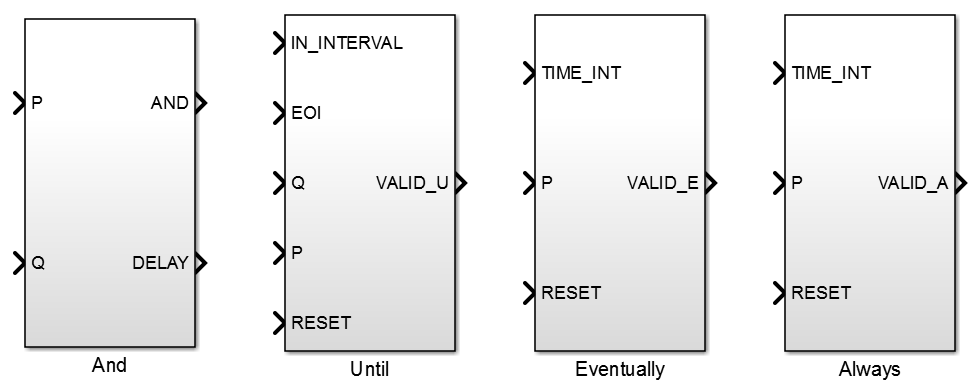
\includegraphics[width=.8\textwidth]{Figs/stlib.PNG} 
     \caption{STL Simulink} 
     \label{fig:stlib} 
\end{figure}
\noindent
\\
The \textit{And} block is needed to implement nested temporal operators, in particular, it represents the conjunction among outer and inner propositions. Despite the name, it is quite different from the classical logical And since it does not returns \textbf{true} if $P$ and $Q$ are \textbf{true} at the same time, but rather if $Q$ becomes \textbf{true} at some the time $t$ after $P$ became \textbf{true}. In order to verify $Q$ it returns, through the $DELAY$ port, the time in which $P$ was verified, such time is needed to correctly compute the interval of the $Q$'s temporal operator.  

\paragraph{} All the operators blocks keep their output constant after a the property is detected. However,  to facilitate their use in simulations concatenating several test cases, a reset input is also provided. Fig. \ref{fig:testSTLALEV} shows two test cases for \textit{Always} and \textit{Eventually}, one causing them return true and one false. 
\begin{figure}[h]
    \centering
    \begin{subfigure}[b]{0.48\textwidth}
        	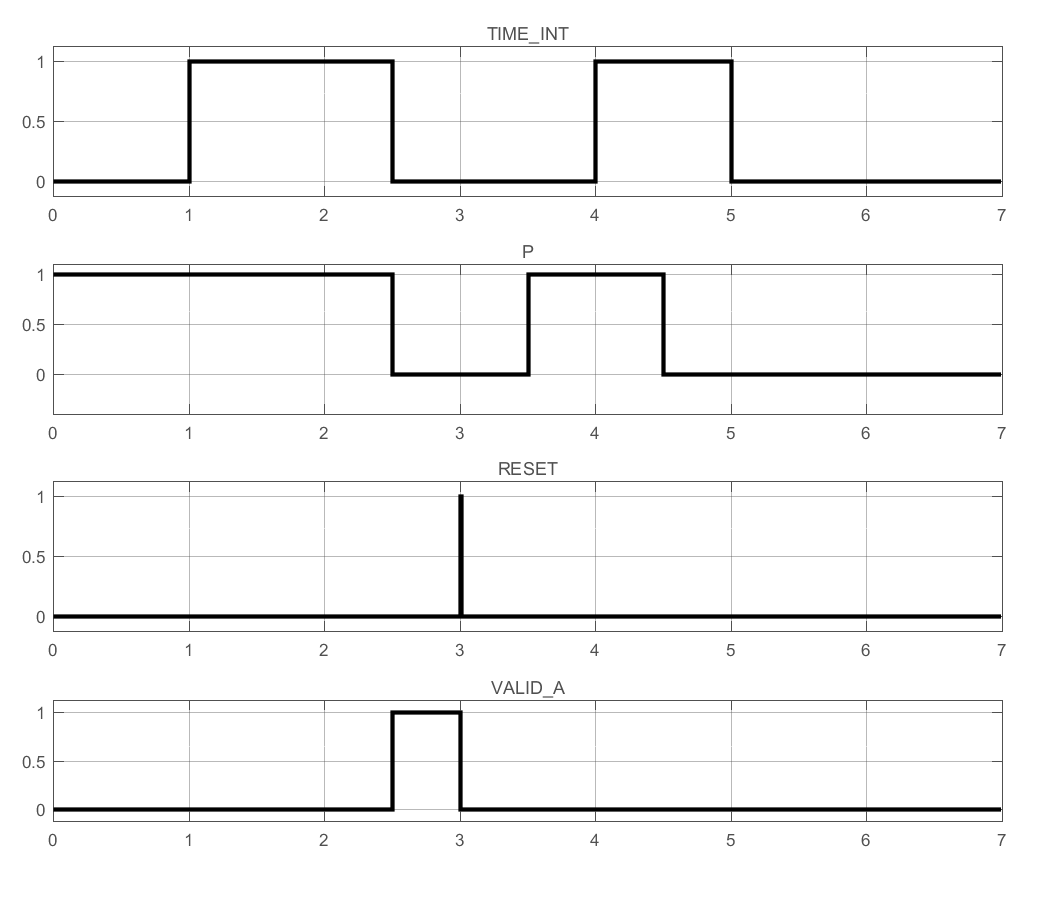
\includegraphics[width=\textwidth,height=188px]{Figs/testalw.eps}
        	\caption{Always}
            \label{fig:testalw}
    \end{subfigure}
        \begin{subfigure}[b]{.48\textwidth}
        	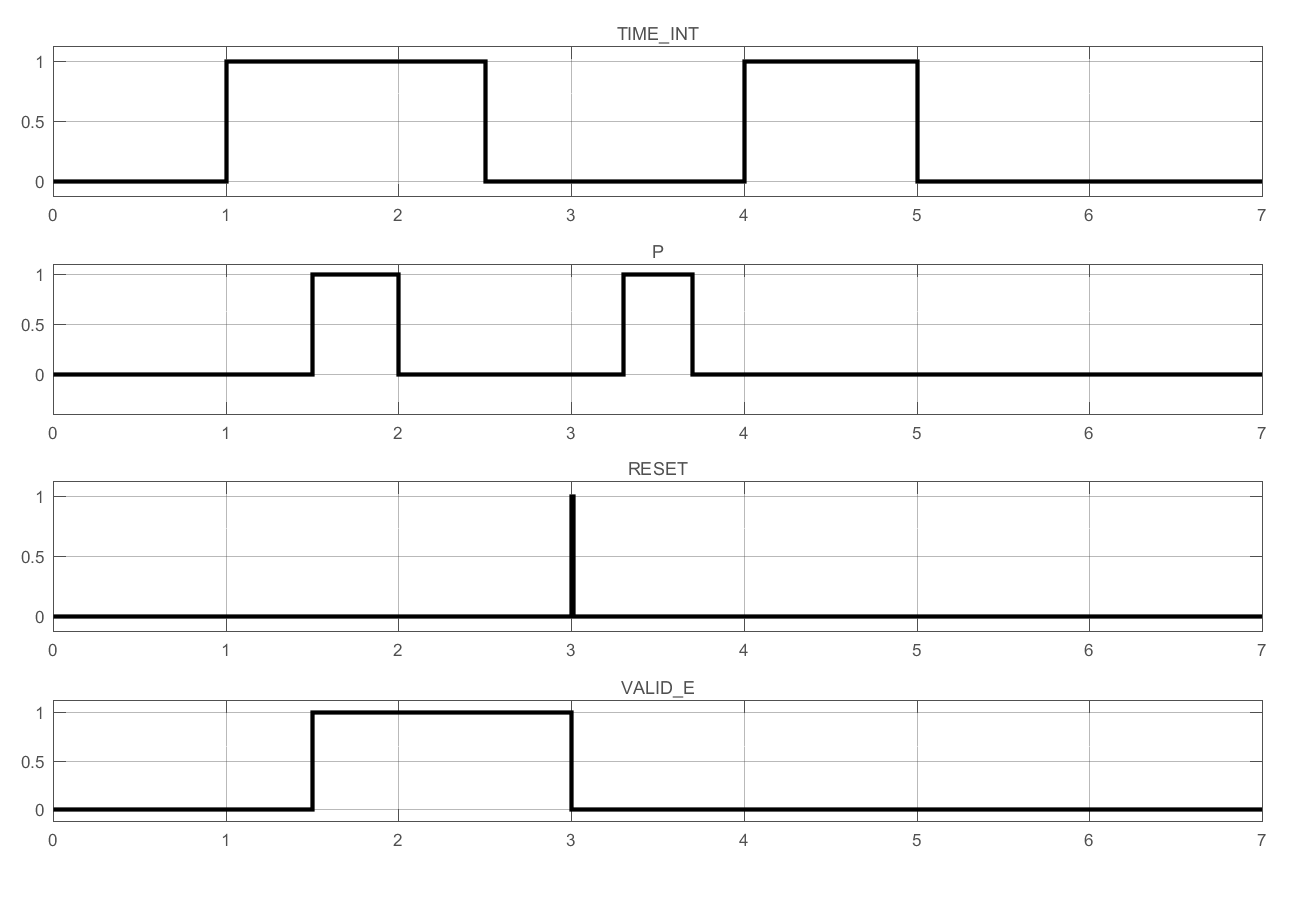
\includegraphics[width=\textwidth,height=188px]{Figs/testev.eps}
        	\caption{Eventually}
            \label{fig:testev}
        \end{subfigure}
    \caption{Test of STL Always-Eventually}
    \label{fig:testSTLALEV}
\end{figure}
\noindent
\\
In particular, it is possible to notice that the two operators have different behaviors due to their dynamics. The Always produces positive outputs only at the end of the time interval relative to the current test case  (Fig.\ref{fig:testalw}). Conversely, the Eventually operator returns positive feedback immediately after the occurrence of a positive input  (Fig.\ref{fig:testev}).
\par Compared to its brothers, the timed \textit{Until} operator has a more complex dynamics, in fact, in presence of multiple test case during the same simulation, it is not possible to determine a priori the instant in which it reacts to each input sequence. Fig. \ref{fig:testunt} present a possible multiple cases simulation for the timed Until.
\begin{figure}[!h]
	\centering
    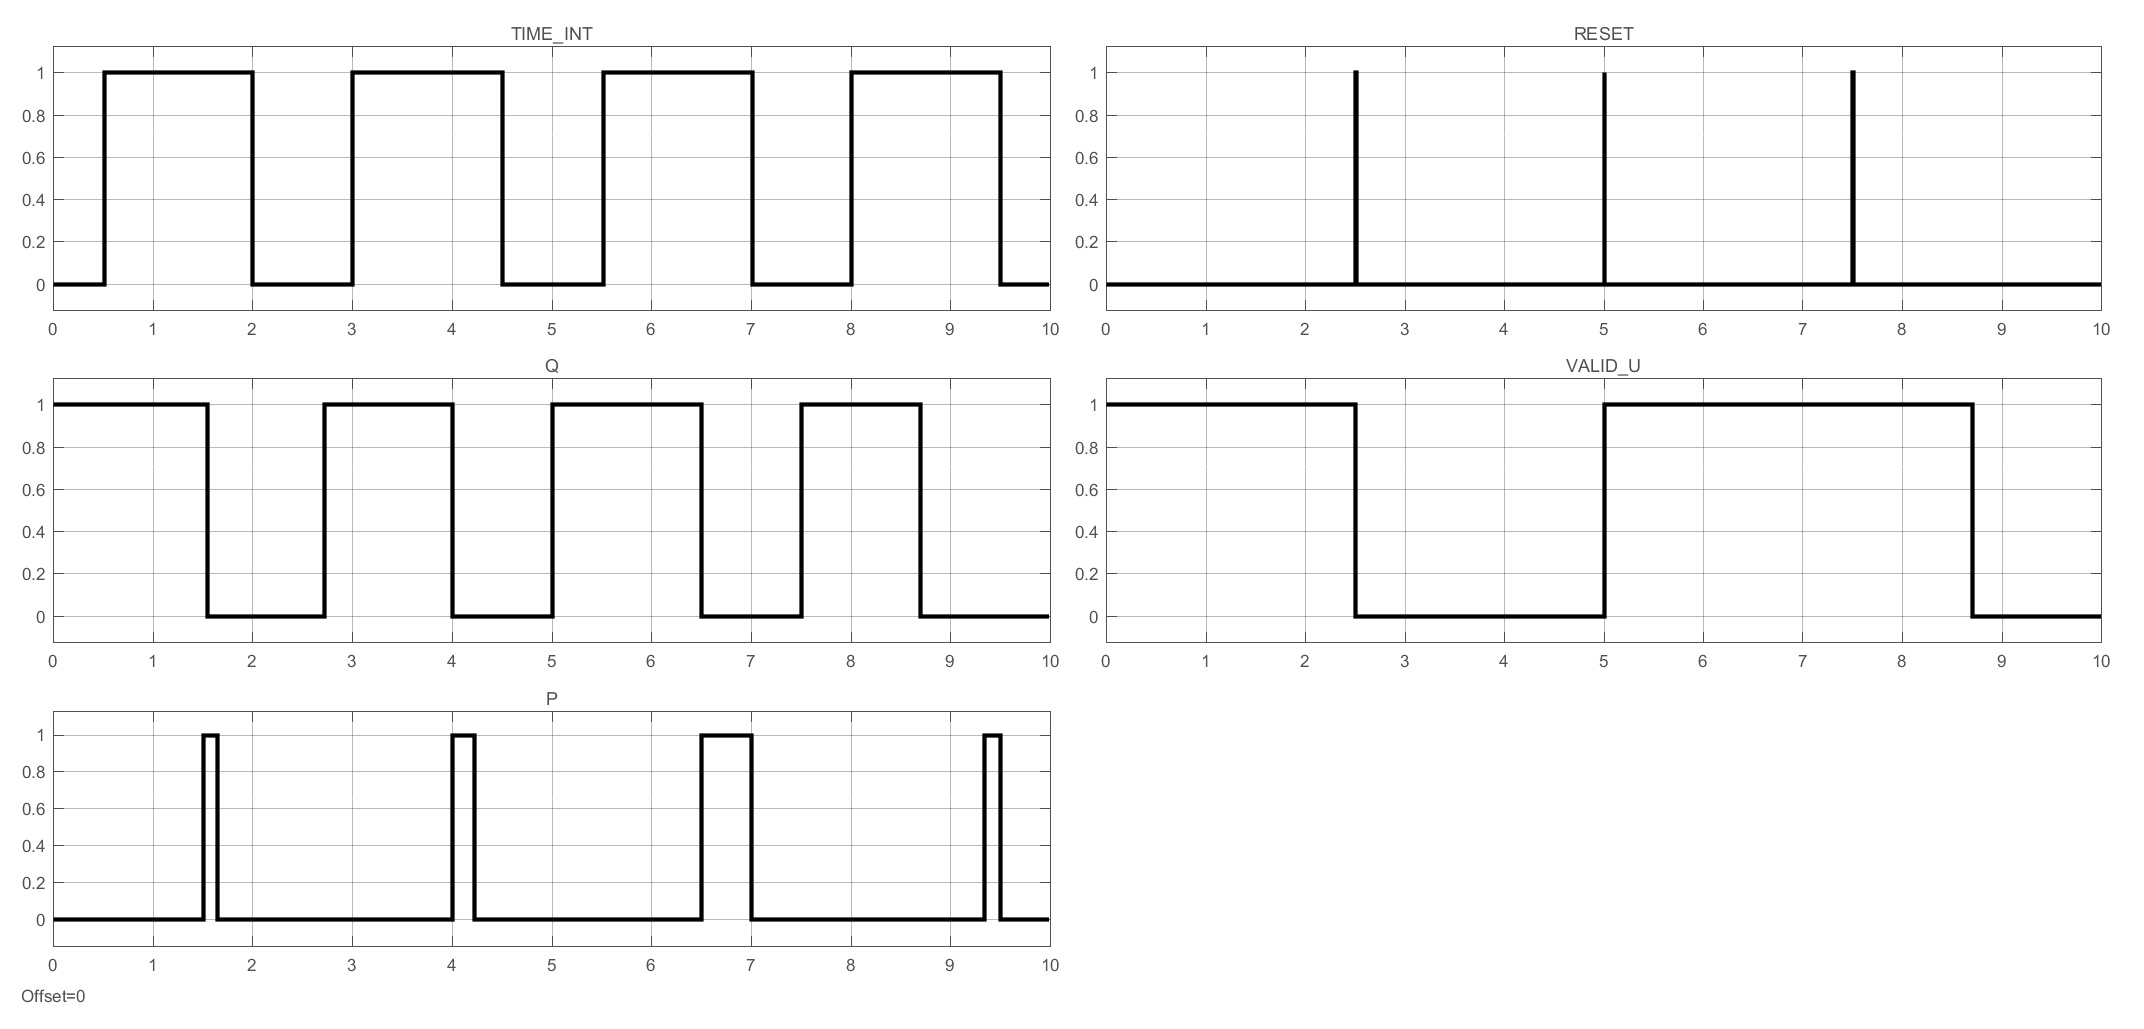
\includegraphics[width=\textwidth]{Figs/testunt.eps}
    \caption{Until Simulation}
    \label{fig:testunt}
\end{figure}
\noindent
\\
The operator returns true if within a time interval the proposition $P$ is true at least once and, for all the time before this happen, the proposition $Q$ is true. The simulation provide four different time intervals. For the first, the operator always returns true since $Q$ is always true until $P$ becomes true. For the second interval, it immediately returns false since, after the reset, the proposition $Q$ is false. After the second pulse of signal reset the operator returns again true, indeed this scenario is perfectly analogous to the first one. During the last time interval, there is yet another behavior. The operator is not immediately returning false, $Q$ is true after the reset, but rather when $Q$ becomes false since $P$ has not yet became true. Note that another behavior, which has not been included for the purpose of not overload the graphics, is observable for the edge case in which $Q$ is always true within a reset and the end of a time interval, and $P$ is always false in the same time. In this case the operator reacts with a negative output only at the end of the time interval, since, till the end , it "waits" for $P$ becoming true.
\paragraph{} The Simulink implementation of the STL timed Until is depicted in Fig. \ref{fig:untimpl}. The other operators are implemented in a similar, and simpler, shape. The complete library is available at \citep{balsrepo}.
\begin{figure}[!h]
\centering
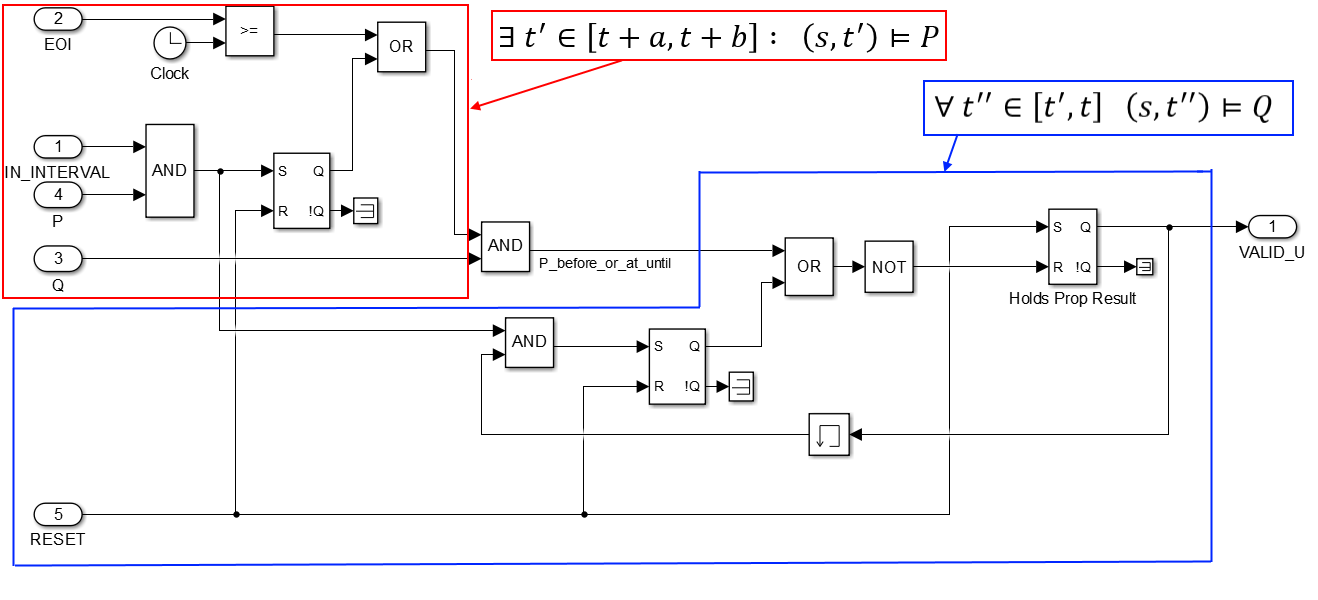
\includegraphics[width=\textwidth]{Figs/untimpl.png}
\caption{Timed Until Implementation}
\label{fig:untimpl}
\end{figure}

\subsection{System Performance Control Library}

Section \ref{ssec:dompatterns} provided an STL formalization of the most common control system performance requirements. In the same has been argued that such formalizations represent patterns, namely parameterizable properties having a fixed formal structure. Offering an implementation of those pattern is the main purpose of the \textit{System Performance Control Library} (SPCL), it provides several atomic blocks able to verify the violation of performance requirements.The library block-set is presented in Fig. \ref{fig:spctrlib}. 

\begin{figure}[h]
\centering
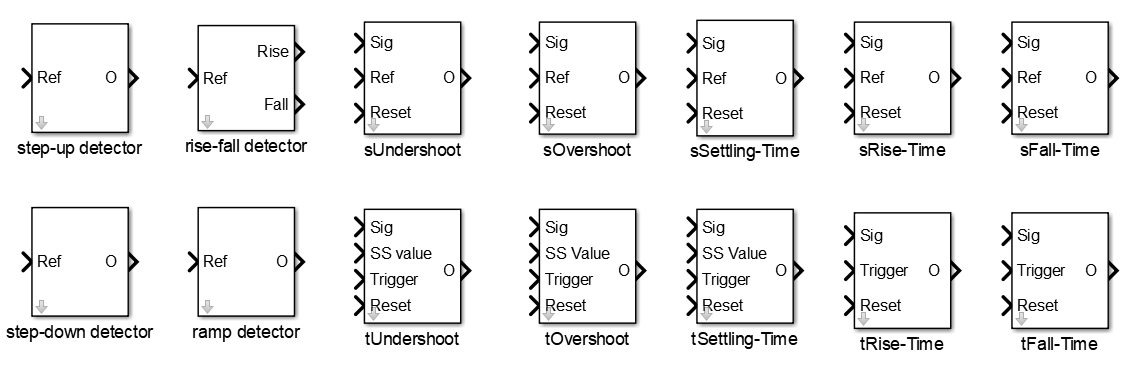
\includegraphics[width=\textwidth]{Figs/spclib.PNG}
\caption{System Performance Control Library}
\label{fig:spctrlib}
\end{figure}

The entire block-set has been developed to operate in a simulation environment that uses a fixed-step solver for \textit{ODE} integration. Possible future versions of the library will eliminate such limitation, allowing their use with a variable-step solver, by simply forcing the user to set a sample time for the block to discretize time and input signals.
\paragraph{} A first categorization of all blocks could be performed by dividing them in \textit{checkers} and \textit{detectors}. Checker blocks, as the name suggest, are those in charge of effectively assert the violation of the property. In order to do so, they need to cooperate with the detectors blocks, which are pulse emitters based on the behavior of their input signals. The cooperation between detectors and checkers can be \textit{implicit} or \textit{explicit}, and allows to split the latter into two more subcategories depending on the type. 
\par Blocks belonging to the first, whose name starts for "\textit{s}", internally perform the classification of the input type by means of a step (up or down) detector. Therefore, those blocks direct implement the formulas of section \ref{ssec:dompatterns}. Ideally this subcategory is enough to verify performance requirements, since these properties are defined under the hypothesis of step as reference input. The reason why the library includes more general versions of this blocks, based on an explicit cooperation with an input detector, comes from the practical user experience. Indeed, many times, along multiple experiments, users may adopt reference signals sharing common features with steps, but having some substantial differences which makes them undetectable as steps. Two common examples are steps followed by a rate limiter (Fig. \ref{fig:ratelim}) and pulse generators (Fig. \ref{fig:pulsegen}). The first is typically used to avoid sharp changes on input and basically transforms a step into a ramp, while the second is used to provide multiple inputs since it can be view as a sequence of up and down steps.  
\begin{figure}[h]
\centering
\begin{subfigure}{\textwidth}
\begin{subfigure}{.48\textwidth}
\centering
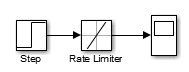
\includegraphics[width=.7\textwidth]{Figs/ratelim2.PNG}
\end{subfigure}
\begin{subfigure}{.48\textwidth}
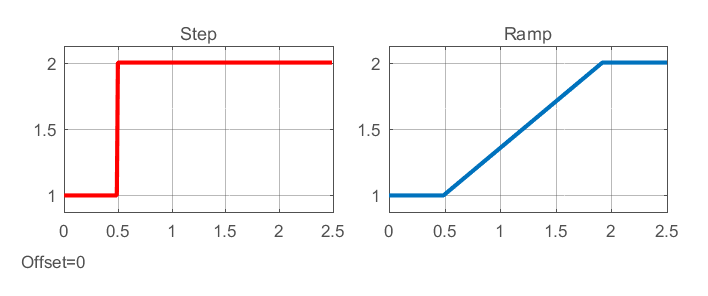
\includegraphics[width=\textwidth]{Figs/ratelimsim.eps}
\end{subfigure}
\caption{Rate Limiter}
\label{fig:ratelim}
\end{subfigure}
\begin{subfigure}{\textwidth}
\begin{subfigure}{.48\textwidth}
\centering
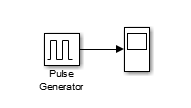
\includegraphics[width=.7\textwidth]{Figs/pulse.PNG}
\end{subfigure}
\begin{subfigure}{.48\textwidth}
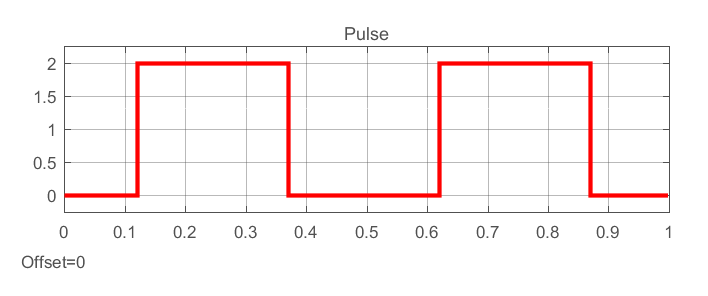
\includegraphics[width=\textwidth]{Figs/pulsesim.eps}
\end{subfigure}
\caption{Pulse Generator}
\label{fig:pulsegen}
\end{subfigure}
\caption{Input References}
\end{figure}
\noindent
\\
In order to support those kind of inputs, without forcing the user to modify existing model to comply with the library, the blocks  family starting with "\textit{t}" label can be used. Unlike the implicit blocks, in addition to the \textit{Trigger} produced by a detector some of them may need more information that normally can be inferred by the reference signal, like, for instance, the steady-state value.

\paragraph{Signal Detectors} As previously said, detectors blocks emit pulses every time the input signal shows an expected behavior. The parameter to evaluate the conditions are set from the user by means of the blocks' masks. In what follows will be focused just the step-up and the ramp detectors, step-down and rise-fall detectors are not considered since the first works reciprocally to the step-up while the second is just a parallel composition of a step-up and a step-down. 
\begin{figure}[h]
\centering
\begin{subfigure}[b]{.48\textwidth}
\centering
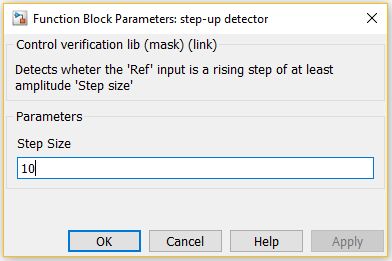
\includegraphics[width=\textwidth]{Figs/stepmask.PNG}
\caption{step-up detector's Mask}
\end{subfigure}
\begin{subfigure}[b]{.48\textwidth}
\centering
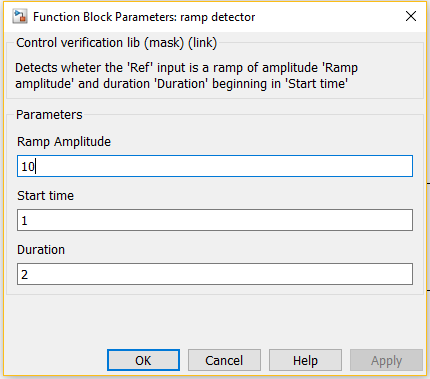
\includegraphics[width=\textwidth]{Figs/rampmask.PNG}
\caption{ramp detector's Mask}
\end{subfigure}
\caption{Detector's masks}
\label{fig:detmasks}
\end{figure}
From the blocks' masks (Fig.\ref{fig:detmasks}) is possible to note that step-up detector, unlike ramp-detector which requires start and duration time, has not parameter which are functions of time, this allow to use it multiple times in the same simulation. A possible time behavior for both detectors is shown in Fig. \ref{fig:detbehavior}, in the case of the step, due to the detectors definition, does not make difference if the input signal is a single step or a step train. Indeed, the detector implementation expects that it reacts every time there is a difference of at least \textit{Step size} between two time-consecutive samples of the input signal.
\begin{figure}[h]
\centering
\begin{subfigure}[b]{.48\textwidth}
\centering
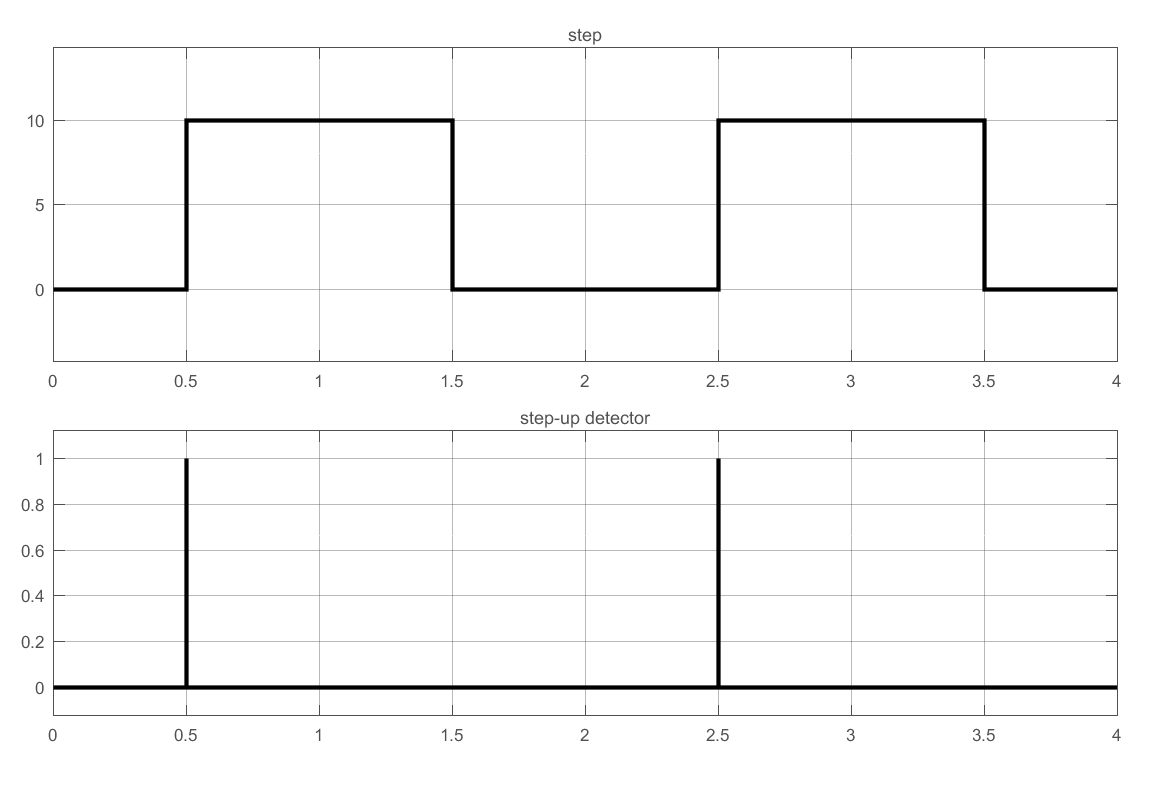
\includegraphics[width=\textwidth]{Figs/stepdetsim.eps}
\end{subfigure}
\begin{subfigure}[b]{.48\textwidth}
\centering
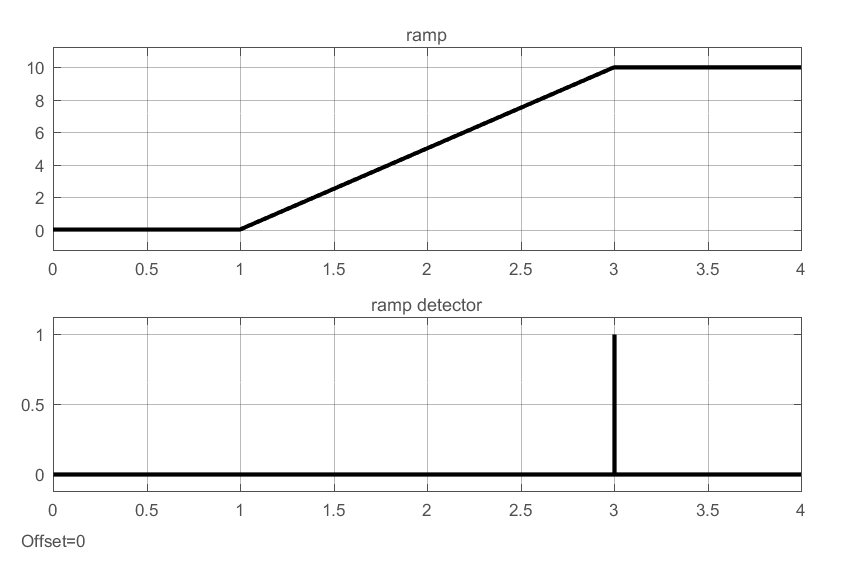
\includegraphics[width=\textwidth]{Figs/rampdetsim.eps}
\end{subfigure}
\caption{Detectors' time behavior}
\label{fig:detbehavior}
\end{figure}
The implementation of the ramp detector is more complex, it is based on the idea that the block must check if, for all $t$ in $[Start, Start+Duration]$, the input signal is a line with a slope equal to $\frac{Amplitude}{Duration}$. This definition can be formally written with the following STL

\begin{center}
$\Box_{[St, St+Dur]}\Bigg\{\dfrac{dx}{dt}==\dfrac{Ampl}{Dur} \Bigg\}$
\end{center}

Such formula can be easily implemented with the Always operator of the STLib (\ref{ssec:STLib}). Please note that in the real implementation (Fig.\ref{fig:rampdetimpl}) the equality of slopes is not checked through the equal operator, but rather ensuring that their difference is less than a very small quantity. This approach has been adopted to avoid possible numerical issues on determining the exact equality of two numbers.
\begin{figure}[ht]
\centering
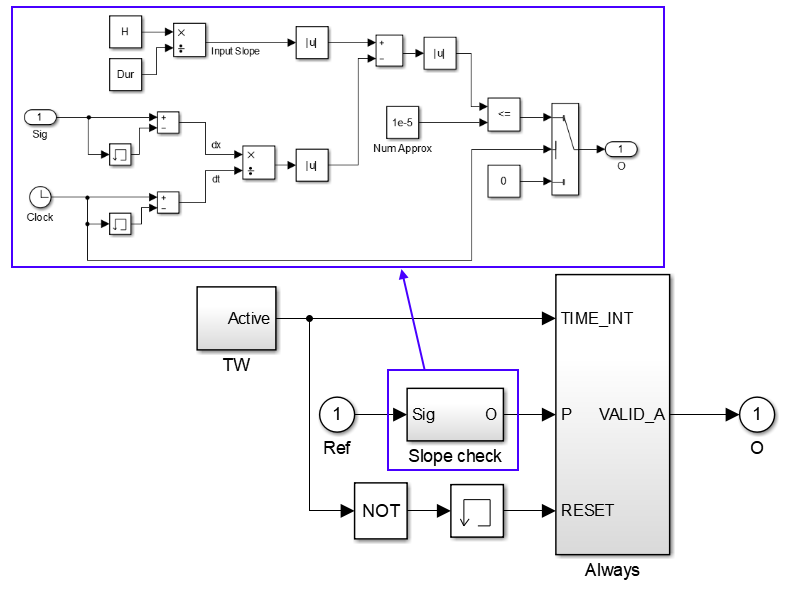
\includegraphics[width=\textwidth]{Figs/rampimpl.png}
\caption{Ramp Detector Implementation}
\label{fig:rampdetimpl}
\end{figure}
\paragraph{Property Checkers} For each performance requirements the library provides two different blocks depending on the type of cooperation with a signal detector. Time behavior and internal structure of blocks-couples relative to each property are very similar. Therefore, without losing generality only overshoot requirement will be analyzed as a case study.
\paragraph{} The property's parameters, provided through the blocks' mask, are slightly different in the case of implicit (Fig.\ref{fig:sovmask}) or explicit (Fig.\ref{fig:tovmask}) reference detection. Indeed, if the blocks has to internally perform the step-up detection it needs to know the step size. Conversely, if the block only receives a detection trigger such parameter is not needed anymore. However, in order for the latter working properly, the information needed to estimate the overshoot has to be provided through a further input port, which has been labeled as "\textit{SS Value}"(Fig.\ref{fig:spctrlib}). The common parameters of the two blocks are \textit{Tolerance}, which represents the maximum tolerated distance among \textit{Sig} and \textit{Ref} (or \textit{SS value}), and \textit{Interval Size}, which corresponds to the simulation time.
\begin{figure}[ht]
\centering
\begin{subfigure}[b]{.4\textwidth}
\centering
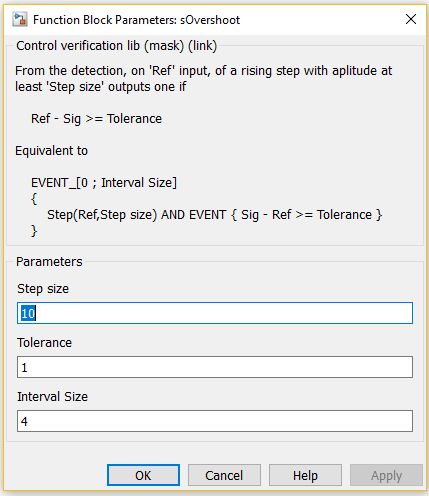
\includegraphics[width=\textwidth]{Figs/sovmask.PNG}
\caption{\textit{sOvershoot}}
\label{fig:sovmask}
\end{subfigure}
\begin{subfigure}[b]{.4\textwidth}
\centering
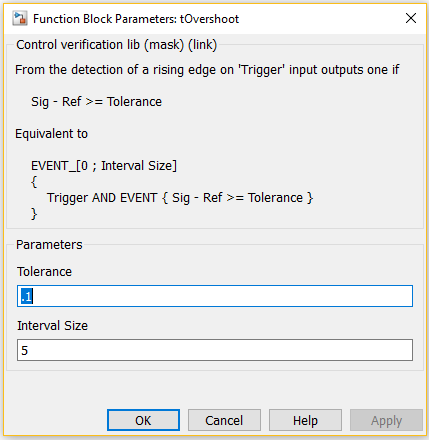
\includegraphics[width=\textwidth]{Figs/tovmask.PNG}
\caption{\textit{tOvershoot}}
\label{fig:tovmask}
\end{subfigure}
\caption{Overshoot Blocks' Masks}
\end{figure}
\paragraph{} Two possible simulations involving \textit{sOvershoot} and \textit{tOvershoot} are shown in Fig.\ref{fig:ovtresp}. For the first a step has been used as reference input, while for the second a ramp. Both blocks reacts immediately after the violation of the requirement.
\begin{figure}[!h]
\centering
\begin{subfigure}[b]{.45\textwidth}
\centering
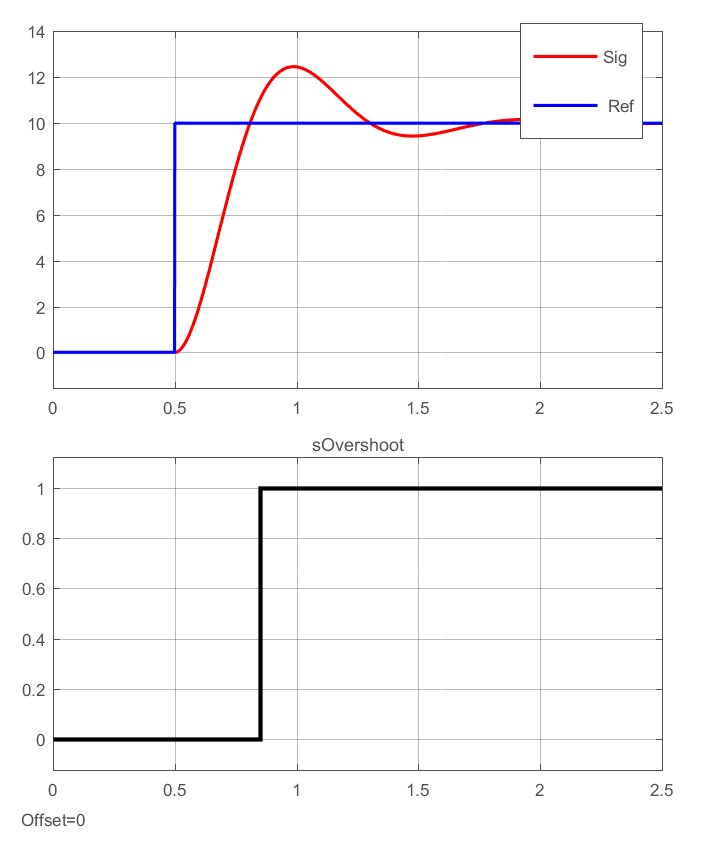
\includegraphics[width=\textwidth]{Figs/sovsim.eps}
\caption{\textit{sOvershoot}}
\end{subfigure}
\begin{subfigure}[b]{.45\textwidth}
\centering
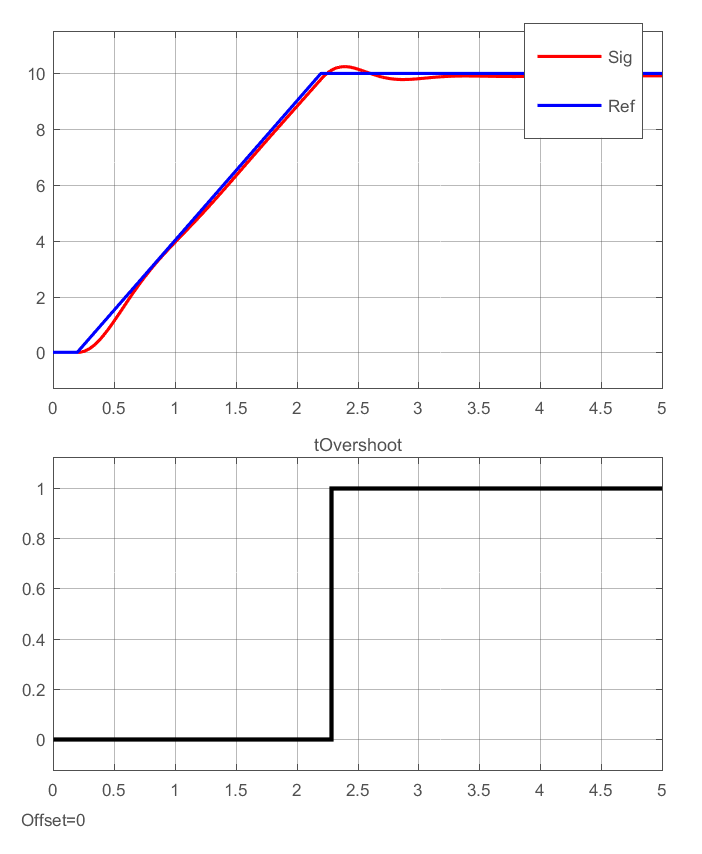
\includegraphics[width=\textwidth]{Figs/tovsim.eps}
\caption{\textit{tOvershoot}}
\end{subfigure}
\caption{Overshoots' Time response}
\label{fig:ovtresp}
\end{figure}
\noindent
\\
The blocks have a layered structure which recalls the level of nesting of the parent STL formula. Essentially, the Simulink implementation of the two blocks only differ for the signal used as first input of the \textit{And} operator inside the blocks' first layer (Fig.\ref{fig:ovimpl}). Such signal correspond to the proposition used at the left of the internal conjunction in nested STL temporal operators. Therefore, the STL formula, implemented in the \textit{tOvershoot} block, can be rewritten as 
\begin{center}
$\lozenge_{[0,T]}\big\{Trigger \wedge \lozenge \{ Sig - SSValue \geq Tolerance\} \big\}$
\end{center}

In order to avoid redundancy, the content of \textit{overshoot} subsystem of Fig.\ref{fig:ovimpl} has not been reported. Indeed, for both versions of the blocks, its structure is analogous to the first layer, i.e. an STL eventually with a less than or equal to proposition as input. 
\begin{figure}[!h]
\centering
\begin{subfigure}[b]{.48\textwidth}
\centering
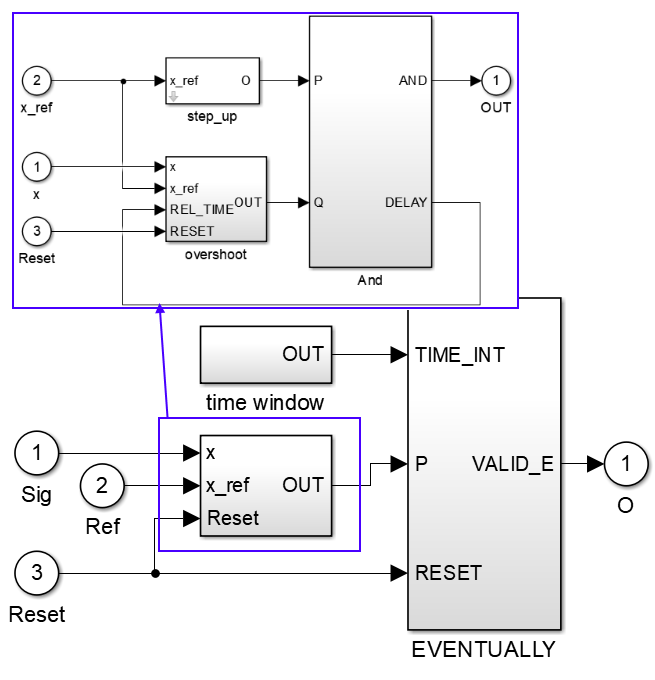
\includegraphics[width=\textwidth]{Figs/sovimpl.png}
\caption{\textit{sOvershoot}}
\end{subfigure}
\begin{subfigure}[b]{.48\textwidth}
\centering
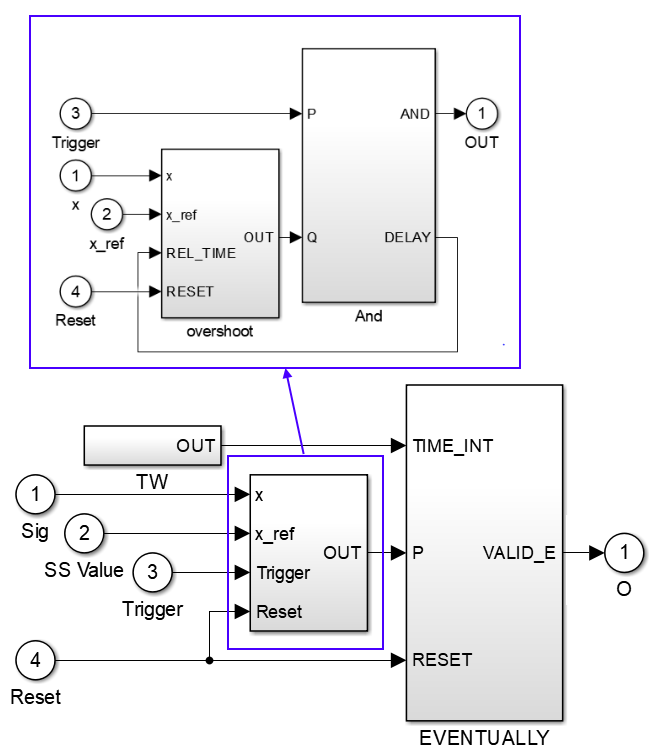
\includegraphics[width=\textwidth]{Figs/tovimpl.png}
\caption{\textit{tOvershoot}}
\end{subfigure}
\caption{Overshoots' Implementations}
\label{fig:ovimpl}
\end{figure}

All other property checkers follow the same philosophy of overshoot blocks. Although with them a good coverage of the performance requirements has been achieved, as future extension other properties may be included, making the \textit{SPCLibrary} a complete tool-chain for the analysis, during simulation, of several control systems models.

\section{Design Patterns}
\label{sec:designpattern}


In object-oriented software design a pattern describes a problem which occurs over and over in the environment, and then describes the core of the solution to that problem, in such a way that you can use this solution multiple times \citep{vlissides1995design}. Design patterns make it easier to reuse successful designs and software architectures, and helps avoiding design alternatives that compromise reusability.
\noindent
\\
Design patterns solve many problems that object-oriented designers face every day, like
\begin{description}
\item[Finding appropriate abjects] The hard part about object-oriented design is decomposing a system into objects. Design patterns help identifying abstractions and the objects that can capture them.
\item[Determining object granularity] Objects can vary tremendously in size and number.Design patterns address this issue as well. Many of them describe specific techniques of decomposing an object into smaller objects.
\item[Specifying object interfaces] Interfaces are fundamental in object-oriented software systems. There is no way to know anything about an object without going through its interface. Design patterns help defining interfaces by identifying their key elements and the kinds of data that get sent across an interface.
\end{description}
\noindent
\\
An exhaustive treatment of all known design patterns requires an huge effort, and leads to cover situation that are out of the scope of this work. Hence, herein only two of them, those really involved, will be taken into consideration. Being scalability and extensibility key factors of the proposed framework, particular care must be payed on the software architecture. The use of patterns belonging to \textit{creational} and \textit{behavioral} classes greatly helps to accomplish this objectives. 

\subsection{Factory}

Creational patterns abstract the instantiation process. They help make a system independent of how its objects are created, composed and represented. A class creational pattern uses inheritance to vary the class that's instantiated, whereas an object creational pattern will delegate instantiation to another object. Creational patterns become important as system evolve to depend more on object composition than class inheritance. As that happens,emphasis shifts away from hard-coding a fixed set of behavior toward defining a smaller set of fundamental behavior that can be composed into any number of more complex ones. Thus creating objects with particular behavior requires more than simply instantiating a class.
\paragraph{} The intent of the \textit{Factory Method} is defining an interface to create objects, but let  decide which class to instantiate. The UML representation of the Factory pattern is shown in Fig.\ref{fig:factory}

\begin{figure}[h]
\centering
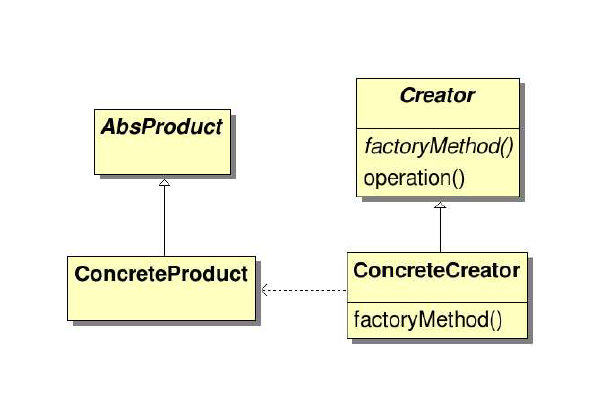
\includegraphics[width=.7\textwidth]{Figs/factory2.png}
\caption{Factory}
\label{fig:factory}
\end{figure}

\begin{description}
\item[Product] defines the interface of the objects the factory method creates
\item[Concrete Product] implements the Product's interface
\item[Creator]declares the factory method
\item[Concrete Creator] overrides the factory method to return an instance of a
ConcreteProduct
\end{description}
\noindent
\\
Sometimes class Factories are implemented as \textit{Singleton}, which is another design pattern ensuring that in the system there is only one instance of the class. The client class request for the creation of new a new concrete product to the Factory and uses object through their interface. Typically the client provide to the Factory a products identifier that is used, for instance, inside a switch/case to determine the correct concrete product to be instantiated. However, managing all possible Concrete Products by hard-coding the logic to create them is not flexible. For this reason, more sophisticated techniques are usually adopted, they make use of the so called \textit{registry} and let Concrete Products register themselves into the factory. Follows a Java implementation example of the Factory pattern, it make use of \textit{Reflections}, which is mechanisms to discover information about the fields, methods and constructors of loaded classes. Further, it allows to use reflected fields, methods, and constructors to operate on their underlying counterparts.

\begin{lstlisting}[language=Java]
interface Product {
	String getName();
}
class ProductOne implements Product {
	static {
		ProductFactory.instance().register("One", ProductOne.class);
	}
	public String getName() { return "instance of ProductOne"; }
    ...		
}
class ProductTwo implements Product {
	static {
		ProductFactory.instance().register("Two", ProductTwo.class);
	}
	public String getName() { return "instance of ProductTwo"; }
    ...	
}

class ProductFactory {
	// Singleton
	static private ProductFactory inst = new ProductFactory();
	static public ProductFactory instance() { return inst; }
	// The registry
	private HashMap registry = new HashMap();
	public void register(String productID, Class productClass) {
		registry.put(productID, productClass);
	}
	public Product create(String ID) {
		Class pClass = (Class)registry.get(ID);
		if (pClass == null) {
			System.err.println("Product " + ID + " not registered");
			return null;
		}
		try {
			Constructor pConstructor = pClass.getDeclaredConstructor(null);
			return (Product)pConstructor.newInstance(null);
		}
}
...
public static void main(String[] args)
{
	Class.forName("ProductOne");
	Class.forName("ProductTwo");
    ...
}
\end{lstlisting}
The Factory uses an associative set in order to couple Concrete Products with their identifier. Each Concrete Product register itself through the initial static block, however, in order to be sure of having all the registration done before start creating Concrete Product, the loader method "\textit{Class.forName(ClassName)}" has to be called.

\subsection{Visitor}
\label{ssec:visitor}

Behavioral patterns are concerned with algorithms and the assignment of responsibility between objects. Behavioral patterns describe not just patterns of objects or classes but also the patterns of communication between them. These pattern characterize complex control flow that's difficult to follow at run-time. They shift the focus away from flow of control to let concentrate just on the way objects are interconnected. 
\paragraph{} \textit{Visitor} pattern uses inheritance to encapsulates behavior that would otherwise be distributed across classes. The intent of the Visitor pattern is to represent an operation to be performed on the elements of an object structure. Visitor lets define new operation without changing the class so the elements on which it operates. In abstract syntax trees, for instance, due to the heterogeneity of nodes' semantic, several distinct operation can be performed. A first approach could be to define an abstract class, \textit{node}, to be the base of an hierarchy of derived class each one implementing a node with a specific semantic \ref{fig:nodehierarchy}.
\begin{figure}[!h]
\centering
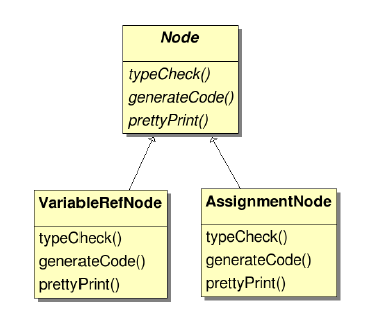
\includegraphics[width=.35\textwidth]{Figs/nodesimple.PNG}
\caption{Node Hierarchy}
\label{fig:nodehierarchy}
\end{figure}
\noindent
\\
The are two main problems of this solution. The first is that the node interface will become too fat in a short time, since all the methods must be part of the interface to be inherited. The second is that the solution does not scale, in fact, if new operations are needed on the node class then the entire hierarchy has to be modified. The Visitor pattern provides a smarter solution which expects to decouple the node structure form its operations, by using additional classes to implement the node visit \ref{fig:visitor}. Then the node class, through the \textit{accept} method, is only providing the "hook" for a generic visitor. \ref{fig:nodeVisitor}

\begin{figure}[h]
\centering
\begin{subfigure}{.48\textwidth}
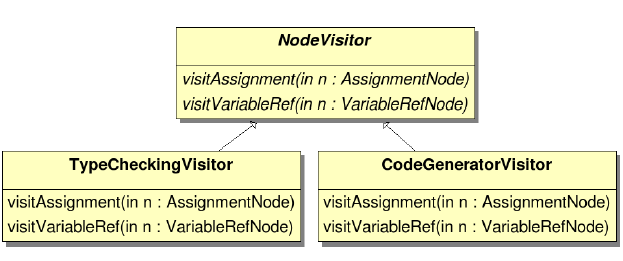
\includegraphics[width=\textwidth]{Figs/visitor.PNG}
\caption{Visitor}
\label{fig:visitor}
\end{subfigure}
\begin{subfigure}{.48\textwidth}
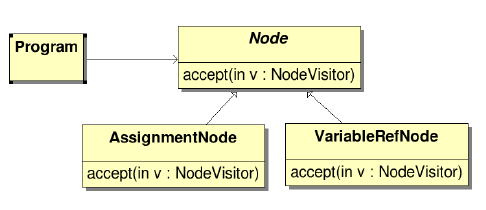
\includegraphics[width=\textwidth]{Figs/nodeVisitor.PNG}
\caption{Node}
\label{fig:nodeVisitor}
\end{subfigure}
\end{figure}

Visitor makes adding new operations easy. It is possible to define new operation over an object structure simply by adding new visitor in contrast to spreading functionality over many classes, which requires to change all of them to define new operation. A visitor gathers related information and separates unrelated ones. Related behavior is not spread over the classes defining the object structure but rather it is localized inside a visitor. However, when using visitor adding new sublasses of node is hard, indeed each new subclass gives rise to a new abstract operation on the visitor, and then require to change all concrete visitors. As partial solution, there could be exceptional cases in which the base visitor provides default implementations that can be inherited from the derived classes. This is the case of ANTLR \citep{antlr}, a popular syntax parser that will be better discussed in \ref{sec:ast}.

\section{Requirements Editor}

The core application of the presented framework is the \textit{Requirements Editor}. It has been implemented as an \textit{Eclipse Editor Plugin}, which provides a set of built-in editing features such as syntax coloring and suggestions engine. The editor is the tool to which the user is directly exposed. It has to provide a user friendly interface and, in the mean time, ensure the construction of well defined requirements. One of the main practical rules for removing entities ambiguities in specifications documents is to use, since the beginning, a Data-Dictionary. It shall contain all the entities referred inside the document, each of them appearing as a record having several explanatory fields. The editor provides support for importing different types of Data-Dictionary (Sec.\ref{sec:datadictimp}).
\par In order to support user in writing syntax coherent requirements the editor provides an helpful engine to \textit{suggest} and \textit{autocomplete} sentences (Sec.\ref{sec:ctxhelper}). They can be also used, especially in the firsts usage attempts, as a mean allowing user to learn the syntax. Such functionality, which are common of many evolved programming editors, are cheap in therms of implementation for formal syntax, but, the more the syntax becomes informal, the more they become expensive. In any case, being extremely difficult comply with all possible inputs combinations, they are usually meant as best-effort tools. 
\par Most likely the main capability of the editor is to allow user to export monitors that can run in several modeling platforms. This is a key feature since allow to save implementation time and  eliminate the presence of interpretation and coding errors. To enforce extensibility the complete process is performed in two steps (Sec.\ref{sec:ast} and \ref{sec:tagetgen}) which are hidden to the user.

\subsection{Data Dictionary Importer}
\label{sec:datadictimp}

Since the Data-Dictionary could be a file of any extension, the importer shall provide support all of them. Hence, the software structure of the importer has to be flexible in order to add, when needed, new file formats. This is a typical problem that software designers solves using the Factory pattern. Each file format needs its own importer, on its own the tool, which has to treat all of them in the same way, it is the only module knowing which importer to instantiate for a specific file. A possible class diagram of the signal readers' software structure is shown in Fig.\ref{fig:ddimpuml}.

\begin{figure}[!h]
\centering
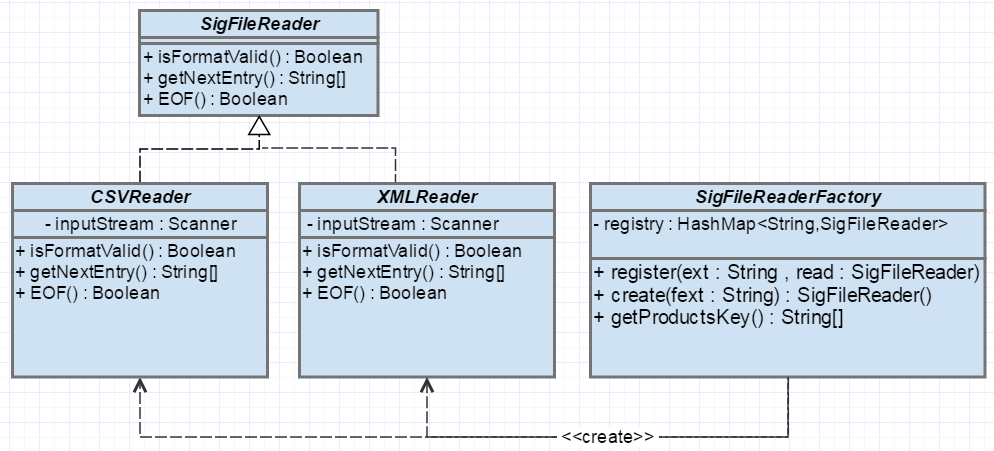
\includegraphics[width=.9\textwidth]{Figs/ddimpUML.PNG}
\caption{Signal Readers UML}
\label{fig:ddimpuml}
\end{figure}
In its first version the importer provides support just for \textit{CSV} and \textit{XML} files, being them common formats for data file. The \textit{SigFileReaderFactory} keeps the supported importers within an associative set, \textit{registry}, which uses as keys the file extension; for instance the key of \textit{CSVFileReader} is ".csv". Using this software structure adding further importers is a quite easy task, in fact it only requires to define the new importer class, e.g. \textit{JSONReader}, deriving from \textit{SigFileReader} and let it call the \textit{SigFileReaderFactory} method \textit{register}. The correct file reader to be instantiated is then determined from the extension of the file provided by the user through the window in Fig.\ref{fig:ddwin}.

\begin{figure}[!h]
\centering
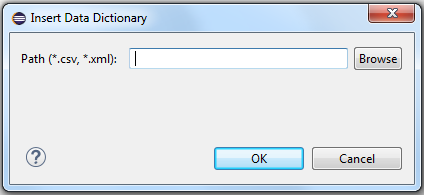
\includegraphics[width=.5\textwidth]{Figs/ddwin.PNG}
\caption{Importer Dialog}
\label{fig:ddwin}
\end{figure}
Through the above dialog is possible to import only files that can be evaluated as Data Dictionaries. Such consistence check is performed through the function \textit{isFormatValid} present in the SigFileReader interface. In particular, such function should provide a positive feedback whether the content of the file is formatted coherently to its extension, and if all of the required fields are present for all the entries of the Data Dictionary. In Fig.\ref{fig:ddcsv} is shown an example of well-formed Data Dictionary.

\begin{figure}[!h]
\centering
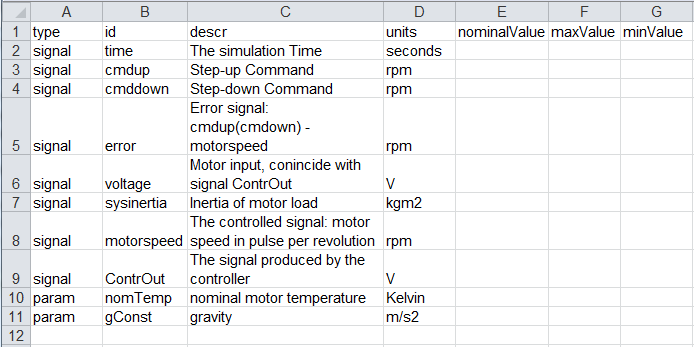
\includegraphics[width=.9\textwidth]{Figs/ddcsv.PNG}
\caption{CSV Data Dictionary}
\label{fig:ddcsv}
\end{figure}
\noindent
\\
It requires the specification of the entry type, its id, two explanatory fields, description and measurement unit, and tree optional numerical values, bounds and nominal value. The same Data Dictionary in XML format is shown in Fig.\ref{fig:ddxml}. 

\begin{figure}[!h]
\centering
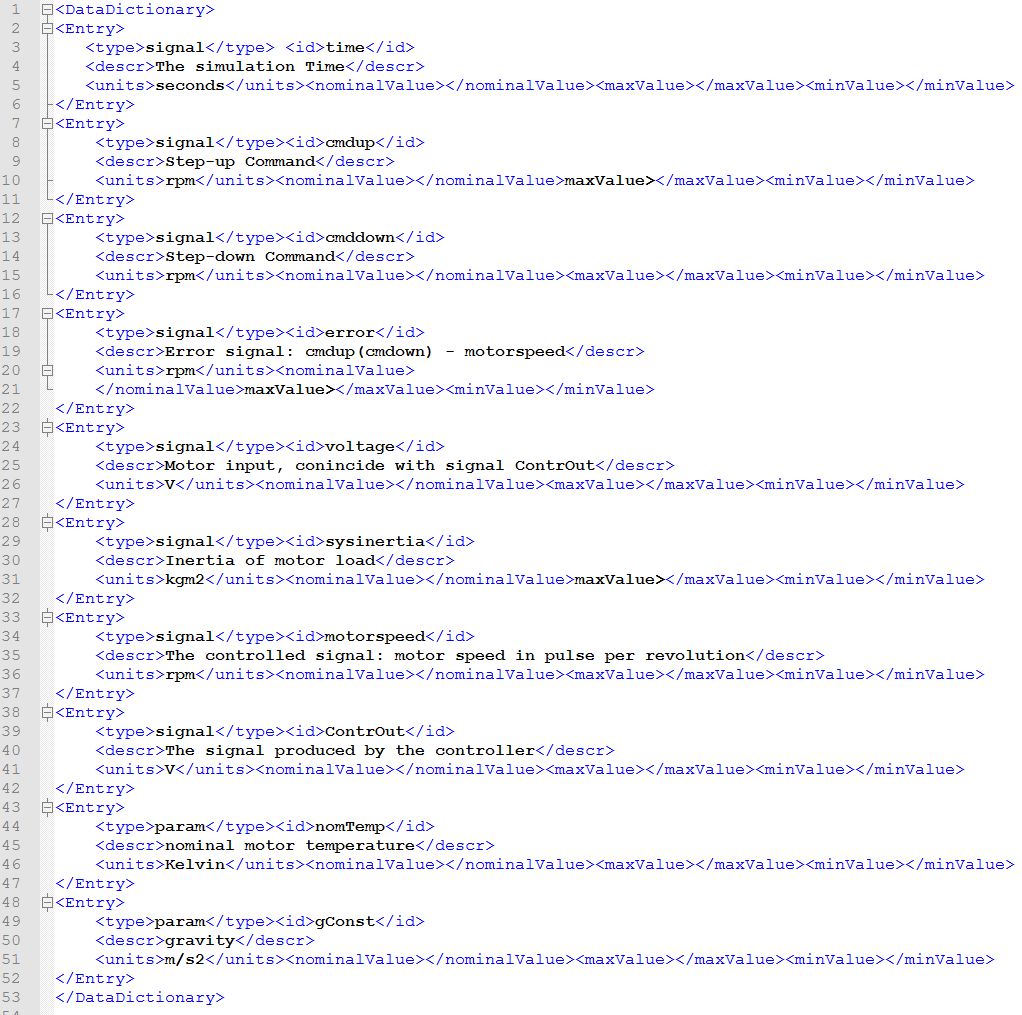
\includegraphics[width=\textwidth]{Figs/ddxml.PNG}
\caption{XML Data Dictionary}
\label{fig:ddxml}
\end{figure}

\subsection{Context Aware Syntax Helper}
\label{sec:ctxhelper}

The Context Aware Syntax Helper provide functionality of word and sentences completion, most commercial editors offer their own such as \citep{IntelliSense}. Typically, whenever the user is typing something and does not remember the exact syntax of what follow, he press a keyword shortcut to invoke the helping engine. The prefix Context Aware is used to clarify that its suggestions varies not only according to the set of keywords preceding the invocation point, but also according the location, in therms of syntax section, on which such point lies. 
\par The context awareness requires to perform kind of hierarchical inspection of the textual "neighborhood" surrounding the invocation point. Then the list of proposals is different according to the syntax section. In other words, it is possible to consider just one syntax for each section and compute a section-wise completion. The syntax defined in \ref{ssec:editorsyn}, can then be partitioned in \textit{Requirement block}, which, in turn, encloses \textit{HEADER}, \textit{ASSUMPTION} and \textit{ASSERTION} (Fig.\ref{fig:reqsec}).

\begin{figure}[!h]
\centering
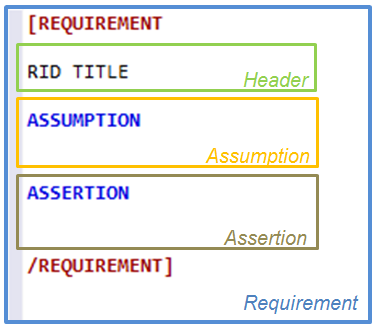
\includegraphics[width=.4\textwidth]{Figs/resec.PNG}
\caption{Syntax Sections}
\label{fig:reqsec}
\end{figure}
Every time the context helper is invoked it determines the current section and provide proposal accordingly. In general, a syntax helper has to behave differently whether it has to provide the completion for an incomplete word or if it has to suggest a continuation after a completed word. For both cases the literature provides an efficient data structure called \textit{Trie} \citep{black2010trie}. A word-Trie is an ordered tree that stores words one character per layer. In Fig.\ref{fig:wtrie} is shown a word-Trie storing the words \textit{"able","ably","aces","aced","babe","bad","back"}.
\begin{figure}[!ht]
\centering
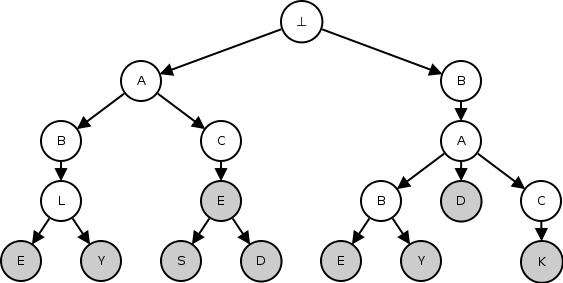
\includegraphics[width=.6\textwidth]{Figs/wtrie.png}
\caption{Word-Trie}
\label{fig:wtrie}
\end{figure}

Typical operations to be performed on Tries are new word insertion and list all possible matching for a partial word. Hence the syntax helper, every time is invoked on an incomplete word, queries a word-Trie to get all possible matching. 
\par A possible generalization of a word-Trie is the sentence-Trie. Instead of storing words per character it stores sentences per words. The insertions policy is quite similar to the one of its simpler version, while the retrieving policy may vary whether one wants to propose just the set of possible following words or possible completion sentences. In the first, case the procedure must return all child nodes of the sentence passed as parameter, while for the second the procedure is the same to the word-Trie and requires to follow all the child path downto the leaves.

\paragraph{} As an example of syntax completion, assume that the user wants to type the following, contract-based, requirement
\begin{center}
\begin{tabular}{ll}
&R.3 Overshoot \\
&\textbf{Assumption:}\\
&system inertia (sysinertia) less than 5 kgm2 \textbf{and} \\
&reference input (cmdup) is a step with amplitude 10\\
&\textbf{Assertion:}\\
&the motor speed (motorspeed) overshoot shall be lass than or equal to 1\\
\end{tabular}
\end{center}
Starting from an empty requirement he types "\textit{system inertia is}" and the invokes the helper, the results returned by the sentence-Trie is all the possible continuing sentences allowed by the syntax of this section.
\begin{figure}[!h]
\centering
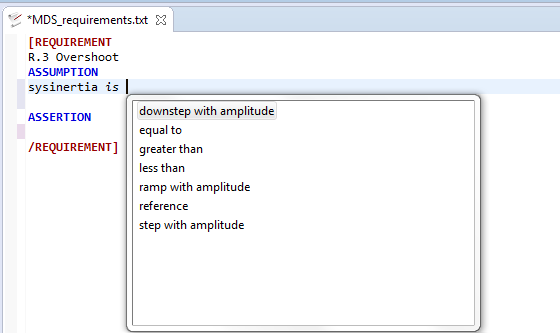
\includegraphics[width=.6\textwidth]{Figs/assumcompl.png}
\caption{Assumption completion}
\label{fig:assumcompl}
\end{figure}
\noindent
\\
In the same manner user can add any number of assumptions, such as the specification of signal generator. The context helper suggest the keyword \textit{"AND"} every time a valid statement has been entered. 

Once all the assumption has been defined, user can switch to the assertion section. In this case, after he inputs the name of the signal, the context helper queries a different sentence-Trie, the one holding the assertions syntax, to provides a different list of completions.
\begin{figure}[h]
\centering
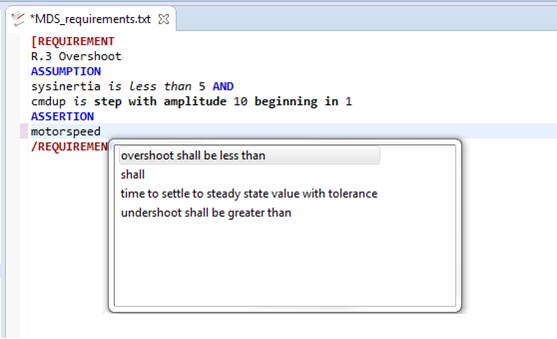
\includegraphics[width=.65\textwidth]{Figs/assercompl.png}
\caption{Assertion completion}
\label{fig:assercompl}
\end{figure}
\noindent
\\
By repeating the above procedure user can type more complex requirements document \ref{fig:reqdoc}, relying on the fact that the syntax he uses is consistent and unambiguous.
\begin{figure}[h]
\centering
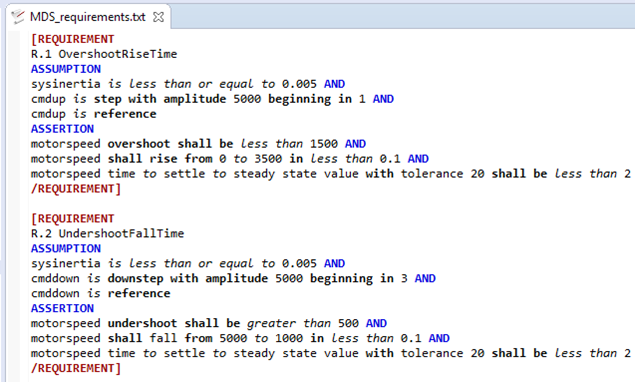
\includegraphics[width=.75\textwidth]{Figs/recdoc.png}
\caption{Requirements Document}
\label{fig:reqdoc}
\end{figure}


\subsection{Abstract Syntax Tree Generation}
\label{sec:ast}

The process of Abstract Syntax Tree Generation is part of the whole generation process. The reason why an intermediate representation is provided is ease the task of platform generators, which does not have to perform any kind of textual analysis. Indeed, an Abstract Syntax Tree has a well defined structure that can be iteratively analyzed and parsed.
\paragraph{} The intermediate representation is achieved involving the grammar parser and lexer ANTLR \citep{antlr}. It allows users to define their own parsable syntax into a  grammar ".g4" file, then it produces a set of classes which are able to recognize the syntax and return the correspondent syntax tree. The process it follows is shown in Fig.\ref{fig:antlrp}

\begin{figure}[!h]
\centering
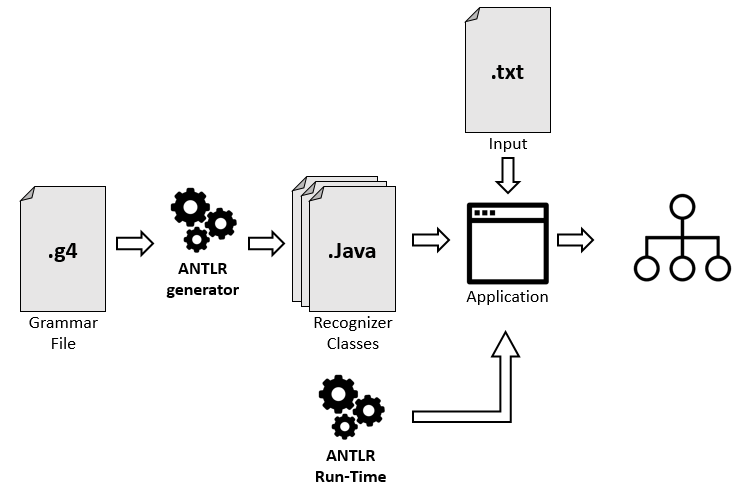
\includegraphics[width=.7\textwidth]{Figs/antlrprocess.PNG}
\caption{ANTLR generation process}
\label{fig:antlrp}
\end{figure}
\noindent
\\
As example, the syntax tree derived from a simple grammar is shown in Fig.\ref{fig:antlrtree}.
\begin{figure}[!h]
\centering
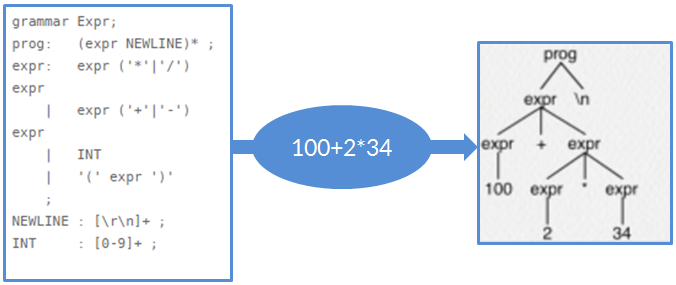
\includegraphics[width=.65\textwidth]{Figs/antlrtree.PNG}
\caption{Basic syntax Example}
\label{fig:antlrtree}
\end{figure}

The generated classes handles the visit of the syntax tree through the Visitor Pattern (Sec.\ref{ssec:visitor}). In particular, if the grammar file is "myGrammar.g4" the two main generated classes are "myGrammarVisitor.java" and "myGrammarBaseVisitor.java". The first corresponds to the visitor interface, while the seconds provides a default implementation of all the nodes' visits. Hence, in order to build its own traversing policy, the user needs to derive the \textit{myGrammarBaseVisitor} class and override the methods performing the visit on the nodes under interest. Alternatively he can define its visitor as a new class which only implements the interface and does not derive from the base visitor, in this case, however, all node visit must be implemented in order to let the new class instantiable.
Input and result of the intermediate transformation are shown in Fig.\ref{fig:reqdoc} and Fig.\ref{fig:intermrepr} respectively. Basically the requirement block keeps it structure, but the requirements are expressed in the following format.
\begin{center}
$PATTERN\_ID(param_1,\dots,param_n)$
\end{center}
This constitutes also the input of the platform generator parser, which is in charge of the translation of patterns into monitors. Note that this structure of the requirements, except for the name, does not provide any information about the pattern, therefore its correct implementation strongly relies on sharing the same pattern semantic between intermediate and platform generators.

\begin{figure}[h]
\centering
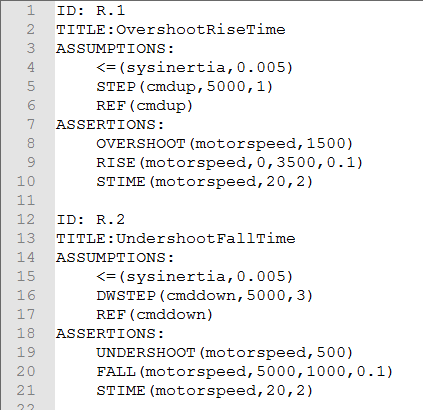
\includegraphics[width=.6\textwidth]{Figs/intermrep.PNG}
\caption{Intermediate Representation}
\label{fig:intermrepr}
\end{figure}

\subsection{Target Platform Generation}
\label{sec:tagetgen}

The target platform is the modeling environment which will hosts the generated monitors. It also has to provide the support for simulation. The platform generator is the module that receives as input a syntax tree and converts its nodes into model's units. Since the generation process is strictly dependent on the modeling environment, it is possible, in the same manner has been done for data-dictionary importers, to associate a specific software module with a specific environment. However, the absence in the syntax tree of environment's features requires to create and treat all generators' classes in the same way. Again this problem is greatly solved by using the Factory design pattern. A possible classes diagrams for a generators hierarchy is shown in Fig.\ref{fig:genuml}

\begin{figure}[h]
\centering
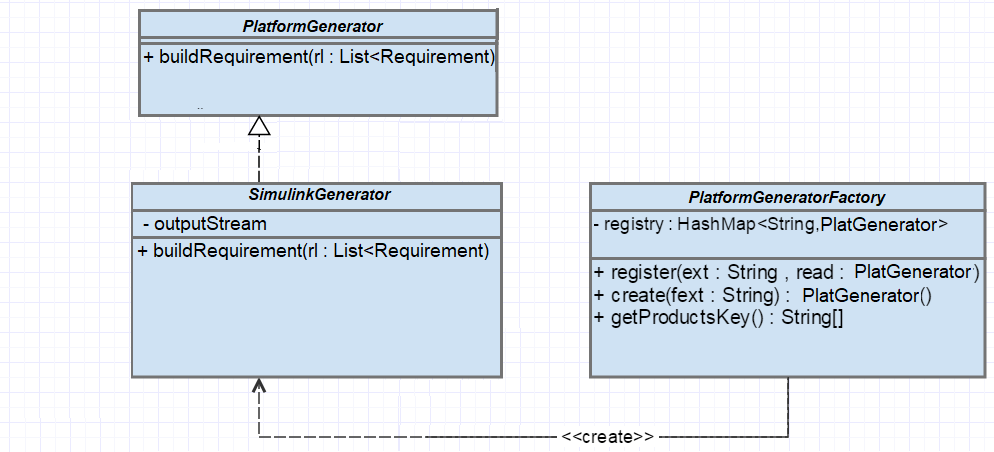
\includegraphics[width=.8\textwidth]{Figs/generatorUML.png}
\caption{Platform Generators UML}
\label{fig:genuml}
\end{figure}
\noindent
\\
A platform generator takes as input a list of requirement and produces a file containing the implementation of the monitors, such a file in the case of Simulink is a Matlab script that, once executed, populates the associated model. 
\par Starting from the requirements document of Fig.\ref{fig:reqdoc}, the user can \textit{build} it through the below window.

\begin{figure}[!h]
\centering
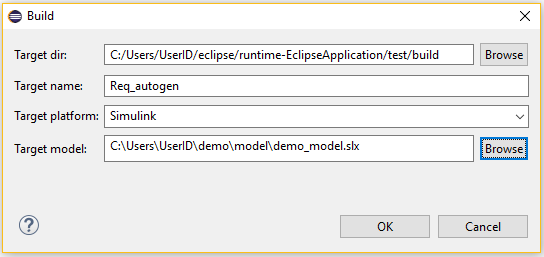
\includegraphics[width=.4\textwidth]{Figs/buildwin.PNG}
\caption{Build Window}
\label{fig:buildwin}
\end{figure}

The \textit{Target Model} field is needed by the generation procedure in order to let the monitor suitable to be attached to the existing model. The other fields are needed in order to, respectively, locate and name the generated script. The result of the model population is shown in Fig.\ref{fig:finalmodel}.

\begin{figure}[h]
\centering
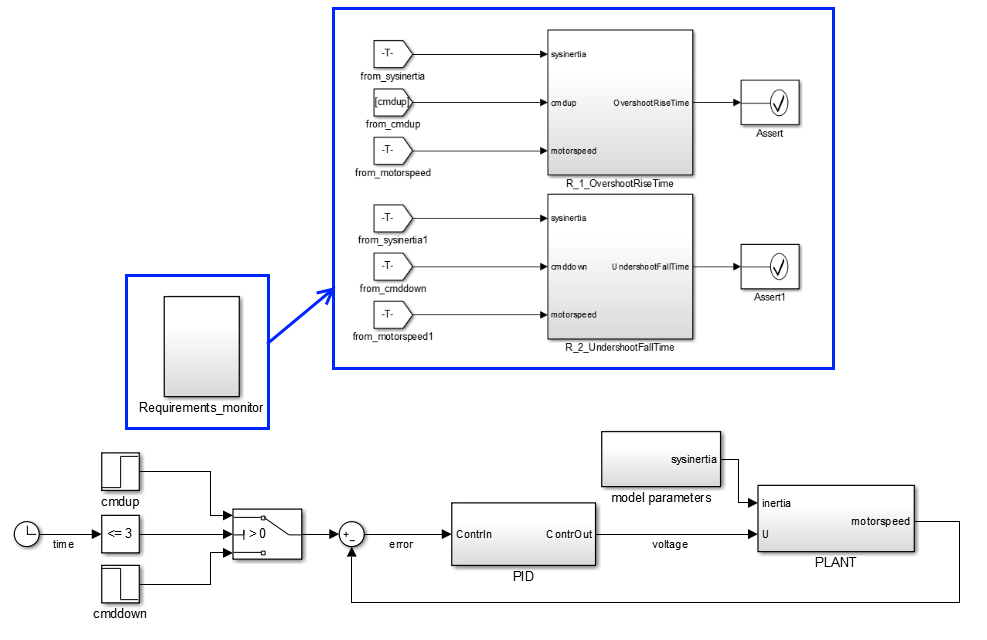
\includegraphics[width=\textwidth]{Figs/finalmodel.png}
\caption{Population Result}
\label{fig:finalmodel}
\end{figure}

The monitor subsystem has as many subsystems as requirements. Each one gets as inputs all the model entities referred inside the requirement and returns an output connected to an assertion block which terminates the simulation if case of false input.

